%%%%%%%%%%%%%%%%%%%%%%%%%%%%%%%%%%%%%%%%
% datoteka diploma-vzorec.tex
%
% vzorčna datoteka za pisanje diplomskega dela v formatu LaTeX
% na UL Fakulteti za računalništvo in informatiko
%
% vkup spravil Gašper Fijavž, december 2010
% 
%
%
% verzija 12. februar 2014 (besedilo teme, seznam kratic, popravki Gašper Fijavž)
% verzija 10. marec 2014 (redakcijski popravki Zoran Bosnić)
% verzija 11. marec 2014 (redakcijski popravki Gašper Fijavž)
% verzija 15. april 2014 (pdf/a 1b compliance, not really - just claiming, Damjan Cvetan, Gašper Fijavž)
% verzija 23. april 2014 (privzeto cc licenca)
% verzija 16. september 2014 (odmiki strain od roba)
% verzija 28. oktober 2014 (odstranil vpisno številko)
% verija 5. februar 2015 (Literatura v kazalu, online literatura)
% verzija 25. september 2015 (angl. naslov v izjavi o avtorstvu)
% verzija 26. februar 2016 (UL izjava o avtorstvu)
% verzija 16. april 2016 (odstranjena izjava o avtorstvu)
% verzija 5. junij 2016 (Franc Solina dodal vrstice, ki jih je označil s svojim imenom)


\documentclass[a4paper, 12pt]{book}
%\documentclass[a4paper, 12pt, draft]{book}  Nalogo preverite tudi z opcijo draft, ki vam bo pokazala, katere vrstice so predolge!
%\def\onlycontent{tru} % comment out to show also the cover pages



\usepackage[utf8x]{inputenc}   % omogoča uporabo slovenskih črk kodiranih v formatu UTF-8
\usepackage[slovene,english]{babel}    % naloži, med drugim, slovenske delilne vzorce
\usepackage[pdftex]{graphicx}  % omogoča vlaganje slik različnih formatov
\usepackage{fancyhdr}          % poskrbi, na primer, za glave strani
\usepackage{amssymb}           % dodatni simboli
\usepackage{amsmath}           % eqref, npr.
%\usepackage{hyperxmp}
\usepackage[hyphens]{url}  % dodal Solina
\usepackage{comment}       % dodal Solina

\usepackage[pdftex, colorlinks=true,
						citecolor=black, filecolor=black, 
						linkcolor=black, urlcolor=black,
						pagebackref=false, 
						pdfproducer={LaTeX}, pdfcreator={LaTeX}, hidelinks]{hyperref}

\usepackage{color}       % dodal Solina
\usepackage{soul}       % dodal Solina
\usepackage[numbers]{natbib}  % dodal Solina

\usepackage{amsthm}
\usepackage{svg}

%%%%%%%%%%%%%%%%%%%%%%%%%%%%%%%%%%%%%%%%
%	DIPLOMA INFO
%%%%%%%%%%%%%%%%%%%%%%%%%%%%%%%%%%%%%%%%
\newcommand{\ttitle}{Digitalna topologija na grafih}
\newcommand{\ttitleEn}{Digital topology on graphs}
\newcommand{\tsubject}{\ttitle}
\newcommand{\tsubjectEn}{\ttitleEn}
\newcommand{\tauthor}{Jakob Drusany}
\newcommand{\tkeywords}{računalnik, računalnik, računalnik}
\newcommand{\tkeywordsEn}{computer, computer, computer}


%%%%%%%%%%%%%%%%%%%%%%%%%%%%%%%%%%%%%%%%
%	HYPERREF SETUP
%%%%%%%%%%%%%%%%%%%%%%%%%%%%%%%%%%%%%%%%
\hypersetup{pdftitle={\ttitle}}
\hypersetup{pdfsubject=\ttitleEn}
\hypersetup{pdfauthor={\tauthor, matjaz.kralj@fri.uni-lj.si}}
\hypersetup{pdfkeywords=\tkeywordsEn}


 


%%%%%%%%%%%%%%%%%%%%%%%%%%%%%%%%%%%%%%%%
% postavitev strani
%%%%%%%%%%%%%%%%%%%%%%%%%%%%%%%%%%%%%%%%  

\addtolength{\marginparwidth}{-20pt} % robovi za tisk
\addtolength{\oddsidemargin}{40pt}
\addtolength{\evensidemargin}{-40pt}

\renewcommand{\baselinestretch}{1.3} % ustrezen razmik med vrsticami
\setlength{\headheight}{15pt}        % potreben prostor na vrhu
\renewcommand{\chaptermark}[1]%
{\markboth{\MakeUppercase{\thechapter.\ #1}}{}} \renewcommand{\sectionmark}[1]%
{\markright{\MakeUppercase{\thesection.\ #1}}} \renewcommand{\headrulewidth}{0.5pt} \renewcommand{\footrulewidth}{0pt}
\fancyhf{}
\fancyhead[LE,RO]{\sl \thepage} 
%\fancyhead[LO]{\sl \rightmark} \fancyhead[RE]{\sl \leftmark}
\fancyhead[RE]{\sc \tauthor}              % dodal Solina
\fancyhead[LO]{\sc Diplomska naloga}     % dodal Solina


\newcommand{\BibTeX}{{\sc Bib}\TeX}

%%%%%%%%%%%%%%%%%%%%%%%%%%%%%%%%%%%%%%%%
% naslovi
%%%%%%%%%%%%%%%%%%%%%%%%%%%%%%%%%%%%%%%%  


\newcommand{\autfont}{\Large}
\newcommand{\titfont}{\LARGE\bf}
\newcommand{\clearemptydoublepage}{\newpage{\pagestyle{empty}\cleardoublepage}}
\setcounter{tocdepth}{1}	      % globina kazala

%%%%%%%%%%%%%%%%%%%%%%%%%%%%%%%%%%%%%%%%
% konstrukti
%%%%%%%%%%%%%%%%%%%%%%%%%%%%%%%%%%%%%%%%  
\newtheorem{izrek}{Izrek}[chapter]
\newtheorem{trditev}{Trditev}[izrek]
\newenvironment{dokaz}{\emph{Dokaz.}\ }{\hspace{\fill}{$\Box$}}

%%%%%%%%%%%%%%%%%%%%%%%%%%%%%%%%%%%%%%%%%%%%%%%%%%%%%%%%%%%%%%%%%%%%%%%%%%%%%%%
%% PDF-A
%%%%%%%%%%%%%%%%%%%%%%%%%%%%%%%%%%%%%%%%%%%%%%%%%%%%%%%%%%%%%%%%%%%%%%%%%%%%%%%


%%%%%%%%%%%%%%%%%%%%%%%%%%%%%%%%%%%%%%%% 
% define medatata
%%%%%%%%%%%%%%%%%%%%%%%%%%%%%%%%%%%%%%%% 
\def\Title{\ttitle}
\def\Author{\tauthor, matjaz.kralj@fri.uni-lj.si}
\def\Subject{\ttitleEn}
\def\Keywords{\tkeywordsEn}

%%%%%%%%%%%%%%%%%%%%%%%%%%%%%%%%%%%%%%%% 
% \convertDate converts D:20080419103507+02'00' to 2008-04-19T10:35:07+02:00
%%%%%%%%%%%%%%%%%%%%%%%%%%%%%%%%%%%%%%%% 
\def\convertDate{%
    \getYear
}

{\catcode`\D=12
 \gdef\getYear D:#1#2#3#4{\edef\xYear{#1#2#3#4}\getMonth}
}
\def\getMonth#1#2{\edef\xMonth{#1#2}\getDay}
\def\getDay#1#2{\edef\xDay{#1#2}\getHour}
\def\getHour#1#2{\edef\xHour{#1#2}\getMin}
\def\getMin#1#2{\edef\xMin{#1#2}\getSec}
\def\getSec#1#2{\edef\xSec{#1#2}\getTZh}
\def\getTZh +#1#2{\edef\xTZh{#1#2}\getTZm}
\def\getTZm '#1#2'{%
    \edef\xTZm{#1#2}%
    \edef\convDate{\xYear-\xMonth-\xDay T\xHour:\xMin:\xSec+\xTZh:\xTZm}%
}

\expandafter\convertDate\pdfcreationdate 

%%%%%%%%%%%%%%%%%%%%%%%%%%%%%%%%%%%%%%%%
% get pdftex version string
%%%%%%%%%%%%%%%%%%%%%%%%%%%%%%%%%%%%%%%% 
\newcount\countA
\countA=\pdftexversion
\advance \countA by -100
\def\pdftexVersionStr{pdfTeX-1.\the\countA.\pdftexrevision}


%%%%%%%%%%%%%%%%%%%%%%%%%%%%%%%%%%%%%%%%
% XMP data
%%%%%%%%%%%%%%%%%%%%%%%%%%%%%%%%%%%%%%%%  
\usepackage{xmpincl}
\includexmp{pdfa-1b}

%%%%%%%%%%%%%%%%%%%%%%%%%%%%%%%%%%%%%%%%
% pdfInfo
%%%%%%%%%%%%%%%%%%%%%%%%%%%%%%%%%%%%%%%%  
\pdfinfo{%
    /Title    (\ttitle)
    /Author   (\tauthor, Jakob Drusany)
    /Subject  (\ttitleEn)
    /Keywords (\tkeywordsEn)
    /ModDate  (\pdfcreationdate)
    /Trapped  /False
}


%%%%%%%%%%%%%%%%%%%%%%%%%%%%%%%%%%%%%%%%%%%%%%%%%%%%%%%%%%%%%%%%%%%%%%%%%%%%%%%
%%%%%%%%%%%%%%%%%%%%%%%%%%%%%%%%%%%%%%%%%%%%%%%%%%%%%%%%%%%%%%%%%%%%%%%%%%%%%%%

\newtheorem{theorem}{Izrek}[section]
\newtheorem{lemma}{Lema}[section]
\newtheorem{corollary}{Posledica}[section]
\theoremstyle{definition}
\newtheorem{definition}{Definicija}[section]
\newtheorem{example}{Primer}[section]
\newtheorem{note}{Opomba}[section]
\theoremstyle{remark}
\newtheorem*{sketch}{Ideja dokaza}

\graphicspath{ {./slike/} }

\begin{document}
\selectlanguage{slovene}
\frontmatter
\setcounter{page}{1} %
\renewcommand{\thepage}{}       % preprecimo težave s številkami strani v kazalu
\newcommand{\sn}[1]{"`#1"'}                    % dodal Solina (slovenski narekovaji)

\ifx\onlycontent\undefined
%%%%%%%%%%%%%%%%%%%%%%%%%%%%%%%%%%%%%%%%
%naslovnica
 \thispagestyle{empty}%
   \begin{center}
    {\large\sc Univerza v Ljubljani\\%
%      Fakulteta za elektrotehniko\\% za študijski program Multimedija
%      Fakulteta za upravo\\% za študijski program Upravna informatika
      Fakulteta za računalništvo in informatiko\\%
      Fakulteta za matematiko in fiziko\\% za študijski program Računalništvo in matematika
     }
    \vskip 10em%
    {\autfont \tauthor\par}%
    {\titfont \ttitle \par}%
    {\vskip 3em \textsc{DIPLOMSKO DELO\\[5mm]         % dodal Solina za ostale študijske programe
%    VISOKOŠOLSKI STROKOVNI ŠTUDIJSKI PROGRAM\\ PRVE STOPNJE\\ RAČUNALNIŠTVO IN INFORMATIKA}\par}%
%     UNIVERZITETNI  ŠTUDIJSKI PROGRAM\\ PRVE STOPNJE\\ RAČUNALNIŠTVO IN INFORMATIKA}\par}%
%    INTERDISCIPLINARNI UNIVERZITETNI\\ ŠTUDIJSKI PROGRAM PRVE STOPNJE\\ MULTIMEDIJA}\par}%
%    INTERDISCIPLINARNI UNIVERZITETNI\\ ŠTUDIJSKI PROGRAM PRVE STOPNJE\\ UPRAVNA INFORMATIKA}\par}%
    INTERDISCIPLINARNI UNIVERZITETNI\\ ŠTUDIJSKI PROGRAM PRVE STOPNJE\\ RAČUNALNIŠTVO IN MATEMATIKA}\par}%
    \vfill\null%
% izberite pravi habilitacijski naziv mentorja!
    {\large \textsc{Mentor}: prof. dr. Petar Pavešić\par}%
%   {\large \textsc{Somentor}:  viš. pred./doc./izr. prof./prof. dr.  Martin Krpan \par}%
    {\vskip 2em \large Ljubljana, 2024 \par}%
\end{center}
% prazna stran
%\clearemptydoublepage      % dodal Solina (izjava o licencah itd. se izpiše na hrbtni strani naslovnice)

%%%%%%%%%%%%%%%%%%%%%%%%%%%%%%%%%%%%%%%%
%copyright stran
\thispagestyle{empty}
\vspace*{8cm}

\noindent
{\sc Copyright}. 
Rezultati diplomske naloge so intelektualna lastnina avtorja in matične fakultete Univerze v Ljubljani.
Za objavo in koriščenje rezultatov diplomske naloge je potrebno pisno privoljenje avtorja, fakultete ter mentorja.

\begin{center}
\mbox{}\vfill
\emph{Besedilo je oblikovano z urejevalnikom besedil \LaTeX.}
\end{center}
% prazna stran
\clearemptydoublepage

%%%%%%%%%%%%%%%%%%%%%%%%%%%%%%%%%%%%%%%%
% stran 3 med uvodnimi listi
\thispagestyle{empty}
\
\vfill

\bigskip
\noindent\textbf{Kandidat:} Jakob Drusany\\
\noindent\textbf{Naslov:} Digitalna topologija na grafih\\
% vstavite ustrezen naziv študijskega programa!
\noindent\textbf{Vrsta naloge:} Diplomska naloga na interdisciplinarnem univerzitetnem programu prve stopnje Raˇcunalniˇstvo in matematika\\
% izberite pravi habilitacijski naziv mentorja!
\noindent\textbf{Mentor:} prof. dr. Petar Pavešić\\

\bigskip
\noindent\textbf{Opis:}\\
Besedilo teme diplomskega dela študent prepiše iz študijskega informacijskega sistema, kamor ga je vnesel mentor. 
V nekaj stavkih bo opisal, kaj pričakuje od kandidatovega diplomskega dela. 
Kaj so cilji, kakšne metode naj uporabi, morda bo zapisal tudi ključno literaturo.

\bigskip
\noindent\textbf{Title:} Digital topology on graphs

\bigskip
\noindent\textbf{Description:}\\
opis diplome v angleščini

\vfill



\vspace{2cm}

% prazna stran
\clearemptydoublepage

% zahvala
\thispagestyle{empty}\mbox{}\vfill\null\it%
\noindent
Na tem mestu zapišite, komu se zahvaljujete za izdelavo diplomske naloge. Pazite, da ne boste koga pozabili. Utegnil vam bo zameriti. Temu se da izogniti tako, da celotno zahvalo izpustite.
\rm\normalfont

% prazna stran
\clearemptydoublepage

%%%%%%%%%%%%%%%%%%%%%%%%%%%%%%%%%%%%%%%%
% kazalo
\pagestyle{empty}
\fi
\def\thepage{}% preprecimo tezave s stevilkami strani v kazalu
\tableofcontents{}
\ifx\onlycontent\undefined


% prazna stran
\clearemptydoublepage

%%%%%%%%%%%%%%%%%%%%%%%%%%%%%%%%%%%%%%%%%
%% seznam kratic
%
%\chapter*{Seznam uporabljenih kratic}  % spremenil Solina, da predolge vrstice ne gredo preko desnega roba
%
%\begin{comment}
%\begin{tabular}{l|l|l}
%  {\bf kratica} & {\bf angleško} & {\bf slovensko} \\ \hline
%  % after \\: \hline or \cline{col1-col2} \cline{col3-col4} ...
%  {\bf CA} & classification accuracy & klasifikacijska točnost \\
%  {\bf DBMS} & database management system & sistem za upravljanje podatkovnih baz \\
%  {\bf SVM} & support vector machine & metoda podpornih vektorjev \\
%  \dots & \dots & \dots \\
%\end{tabular}
%\end{comment}
%
%\noindent\begin{tabular}{p{0.1\textwidth}|p{.4\textwidth}|p{.4\textwidth}}    % po potrebi razširi prvo kolono tabele na račun drugih dveh!
%  {\bf kratica} & {\bf angleško}                             & {\bf slovensko} \\ \hline
%  {\bf CA}      & classification accuracy               & klasifikacijska točnost \\
%  {\bf DBMS} & database management system & sistem za upravljanje podatkovnih baz \\
%  {\bf SVM}   & support vector machine              & metoda podpornih vektorjev \\
%%  \dots & \dots & \dots \\
%\end{tabular}


% prazna stran
%\clearemptydoublepage

%%%%%%%%%%%%%%%%%%%%%%%%%%%%%%%%%%%%%%%%
% povzetek
\addcontentsline{toc}{chapter}{Povzetek}
\chapter*{Povzetek}

\noindent\textbf{Naslov:} \ttitle
\bigskip

\noindent\textbf{Avtor:} \tauthor
\bigskip

%\noindent\textbf{Povzetek:} 
\noindent V vzorcu je predstavljen postopek priprave diplomskega dela z uporabo okolja \LaTeX. Vaš povzetek mora sicer vsebovati približno 100 besed, ta tukaj je odločno prekratek.
Dober povzetek vključuje: (1) kratek opis obravnavanega problema, (2) kratek opis vašega pristopa za reševanje tega problema in (3) (najbolj uspešen) rezultat ali prispevek magistrske naloge.

\bigskip

\noindent\textbf{Ključne besede:} \tkeywords.
% prazna stran
\clearemptydoublepage

%%%%%%%%%%%%%%%%%%%%%%%%%%%%%%%%%%%%%%%%
% abstract
\selectlanguage{english}
\addcontentsline{toc}{chapter}{Abstract}
\chapter*{Abstract}

\noindent\textbf{Title:} \ttitleEn
\bigskip

\noindent\textbf{Author:} \tauthor
\bigskip

%\noindent\textbf{Abstract:} 
\noindent This sample document presents an approach to typesetting your BSc thesis using \LaTeX. 
A proper abstract should contain around 100 words which makes this one way too short.
\bigskip

\noindent\textbf{Keywords:} \tkeywordsEn.
\selectlanguage{slovene}
% prazna stran
\clearemptydoublepage
\fi
%%%%%%%%%%%%%%%%%%%%%%%%%%%%%%%%%%%%%%%%
\mainmatter
\setcounter{page}{1}
\pagestyle{fancy}

\chapter{Uvod}
Procesiranje slik je zelo pomembna in hitro rastoča veja računalništva z 
obširno uporabo na različnih področjih, recimo avtomatizirano branje dokumentov
v poslovnem svetu, avtomatski nadzor kakovosti v proizvodnji, medicinska diagnostika
na podlagi radiologije ipd. To delo bo osredotočeno na analizo slik.
Za dano sliko hočemo pridobiti njen opis na podlagi objektov in regij na njej
in njihovih medsebojnih relacij. Recimo dokument je sestavljen iz znakov na nekem ozadju, krvni razmaz je 
sestavljen iz krvnih celic na nekem ozadju, rentgenska slika je sestavljena
iz različnih organov itd. Prva faza procesiranja je torej ločevanje slike na
različne regije -- na objekte v ospredju in ozadje. Ta proces imenujemo \textbf{segmentacija}.\\
Segmentacija je postopek dodeljevanja vsakega slikovnega elementa (piksla) v enega ali več
razredov. Eden izmed preprostih pristopov je binarna segmentacija, kjer sliko razdelimo
na dve regiji, ozadje in ospredje, na podlagi izbranega praga. Če je svetlost piksla večja
od tega praga, ga dodelimo v ospredje, sicer pa v ozadje, ali obratno. Obstaja veliko več
kompleksnejših metod segmentacije, ki uporabljajo več podatkov kot samo svetlost
pikslov.\\
Ko sliko enkrat segmentiramo v manjše regije, lahko začnemo analizirati lastnosti
teh regij in njihove medsebojne relacije. Nekatere lastnosti so odvisne od svetlosti
pikslov, druge samo od pozicije pikslov. Zelo osnovne so topološke lastnosti
regij, ki vključujejo koncepte, kot so povezanost in sosednost, in so neodvisne od
velikosti in oblike regij.\\
Topološke lastnosti so uporabne zaradi različnih razlogov. Po tem, ko smo izbrali
neko regijo, recimo ospredje dokumenta, jo ponavadi hočemo še segmentirati v
manjše povezane regije. Te predstavljajo posamezne objekte, kot so znaki na dokumentu. Lahko
hočemo skrčiti regijo na okostje, ki predstavlja skrčeno obliko regije in ohranja
povezanost.
V večini literature se sliko predstavi kot neke vrste graf. Ponavadi je tak, da
so vozlišča piksli, vozlišči pa sta povezani, če sta sosednji (bodisi 4-povezanost
bodisi 8-povezanost). Opazovanje topoloških lastnosti slik torej porodi potrebo po
raziskovanju topologij na grafih.

\section{Teoretične osnove}
Vsi omenjeni grafi bodo neusmerjeni, brez izoliranih vozlišč in enostavni (brez zank
in večkratnih povezav med vozlišči).
\textbf{Graf} $G = (V,E)$ je določen z množico vozlišč $V$ in množico povezav $E \subseteq \binom{V}{2}$.
Povezavo $\{x,y\} \in E,\ x,y \in V$, lahko označimo tudi z $xy$.\\
Množico sosednjih vozlišč vozlišča $x$ označujemo z \[N_x = \{y \in V\ |\ xy \in E\}.\]\\
Število sosednjih vozlišč vozlišča $x$ je \[\deg(x) = |N_x|.\] Če je $\deg(x)$ končno
za vsak $x \in V$, je graf $G$ \textbf{lokalno končen}.\\
$G$ je \textbf{povezan graf}, če za vsak par vozlišč $x,y \in V$ obstaja končno
zaporedje različnih vozlišč $v_1,\ \dots,\ v_n \in V$, da velja \[xv_1,\ v_1v_2,\ \dots,\ v_n y \in E.\]\\
Graf $G$ imenujemo \textbf{cikel}, če je $V$ končna množica $n$ točk \[V=\{v_1,\dots,v_n\}\] in
\[E=\{v_1 v_2,\ \dots,\ v_{n-1}v_n,\ v_n v_1\}.\] \\
Za vsako množico vozlišč $V' \subseteq V$ definiramo \textbf{induciran podgraf} \[G[V'] = (V',E'),\]
kjer je \[E' = \{xy \in E\ |\ x,y \in V'\}.\] Induciran podgraf potemtakem ohranja vse povezave
iz $G$, ki povezujejo vozlišča iz $V'$. Če je $G'$ induciran podgraf $G$,
ga označimo z relacijo $G' \sqsubseteq  G$.\\
Množico vozlišč grafa $G$ označimo z $V(G)$, množico povezav pa z $E(G)$. Unija
grafov $G_1 \cup G_2$ je definirana kot graf, ki ima vozlišča $V(G_1) \cup V(G_2)$
in povezave $E(G_1) \cup E(G_2)$.\
\textbf{Orientacija} grafa $G$ je taka šibka urejenost (refleksivna in tranzitivna relacija)
na množici vozlišč $V(G)$, da velja $xy \in E(G)$, če in samo če je $x < y$ ali $y < x$.\\\par
\textbf{Topologija} (ali topološka struktura) na množici $X$ je družina $\mathcal{T}$ podmnožic
$X$, ki zadošča naslednjim zahtevam:
\begin{itemize}
    \item[(1)] prazna množica in $X$ sta elementa $\mathcal{T}$;
    \item[(2)] unija poljubne poddružine $\mathcal{T}$ je element $\mathcal{T}$;
    \item[(3)] presek poljubne končne poddružine $\mathcal{T}$ je element $\mathcal{T}$.
\end{itemize}
Elemente $\mathcal{T}$ imenujemo \textbf{odprte množice} v $X$. \textbf{Topološki prostor}
($X$, $\mathcal{T}$) je množica $X$, opremljena s topologijo $\mathcal{T}$.\\
\textbf{Okolica} točke $x \in X$ je vsaka podmnožica $V \subseteq X$, ki vsebuje
odprto množico $U$, ki vsebuje $x$.\\
Premislimo kaj so ekstremne možnosti za topologijo na $X$.
Najmanj, kar mora vsebovati sta prazna množica in $X$. Hitro lako preverimo, da
je to topologija, pravimo ji \textbf{trivialna topologija}. Na drugi strani,
lahko vzamemo vse podmnožice $X$ kot odprte množice. To je \textbf{diskretna topologija}.
Družina odprtih množic je \textbf{baza} topologije prostora $(X,\mathcal{T})$, če 
vsak element $\mathcal{T}$ lahko izrazimo kot unijo množic iz baze.\\
Topološki prostor je \textbf{povezan}, če se množice $X$ ne da izraziti kot unije
dveh disjunktnih nepraznih odprtih množic.\\
Funkcija $f:\ (X,\mathcal{T}) \rightarrow (X',\mathcal{T}')$ je \textbf{homeomorfizem}, če je
$f:\ X \rightarrow X'$ bijektivna, ter če $f$ inducira bijekcijo med $\mathcal{T}$ in $\mathcal{T}'$.
Tedaj pravimo, da sta topološka prostora $(X,\mathcal{T})$ in $(X',\mathcal{T}')$ \textbf{homeomorfna}.\\
\textbf{Topologija Aleksandrova} je topologija, v kateri je vsak presek odprtih
množic odprt (v navadni topologiji to velja samo za končne preseke). Presek vseh odprtih množic, 
ki vsebujejo točko $x$ je torej \textbf{najmanjša odprta okolica} točke $x$, ki jo označimo z $U_x$.\\
Za topologijo $\mathcal{T}$ na množici $X$ pravimo, da \textbf{loči} podmnožico $A \subseteq X$
od podmnožice $B \subset X$, če obstaja odprta množica $U$, ki vsebuje $A$ in ne vsebuje $B$,
torej $A \subseteq U$ in $B \cap U = \emptyset$. Topologija \textbf{ostro loči}, če obstajata
$U,V \in \mathcal{T}$, da velja $A \subseteq U, B \subseteq V$ in $U \cup V = \emptyset$ \\
\textbf{Aksiomi ločljivosti} so zahteve za topološki prostor, ki zagotavljajo določeno
stopnjo ločljivosti med točkami. Pišemo jih kot zaporedje vedno ostrejših zahtev
$T_0,\ T_1,\ T_2,\ T_3,\ T_4$.\\

\begin{itemize}
  \item[$X$] je $T_0$: Za različni točki $x,y \in X$ obstaja odprta množica $U$, ki vsebuje
  eno in ne drugo točko.
  \item[$X$] je $T_1$: Za različni točki $x,y \in X$ obstaja okolica točke $x$, ki jo
  ostro loči od $y$ in obenem obstaja okolica točke $y$, ki jo ostro loči od $x$.
\end{itemize}

Ostali aksiomi v tem delu niso pomembni, saj se bomo osredotočali na končne
topološke prostore. \textbf{Končna} topologija je topologija na končni množici. Vsaka končna
topologija je topologija Aleksandrova in brž ko zahtevamo na takem prostoru
$T_1$, se nam porodi diskretna topologija.

\chapter{Končne topologije, delne urejenosti in celični kompleksi}
\section{Povezava končnih topologij in delnih urejenosti}\label{poset-top}
Šibko urejena množica je množica s tranzitivno in refleksivno relacijo.
Pokazali bomo, da poljubna končna topologija na $X$ porodi šibko urejenost na $X$ in obratno.
Dovolj je že, če je ta topologija topologija Aleksandrova.\\
Minimalne odprte množice vseh točk tvorijo bazo prostora,
saj je vsaka odprta množica $U \subseteq X$ unija minimalnih odprtih množic $U_x,\ x\in U$.
Bazi, ki je sestavljena iz minimalnih odprtih množic pravimo minimalna baza.
Vsaka baza prostora vsebuje minimalno bazo,
ker če izrazimo $U_x$ kot unijo odprtih množic iz baze, mora ena od teh množic
vsebovati $x$. Tedaj ta množica sovpada z $U_x$.\\
Naj bo $X$ topološki prostor z bazo $\{U_x\}_{x \in X}$. Na množici $X$ definiramo
relacijo le s pravilom:
\[x \leq y\quad \Longleftrightarrow\quad x \subseteq y\]
Podana relacija je šibka urejenost nad $X$. Obratno, iz šibke urejenosti
definiramo topologijo nad $X$ z bazo $\{y \in X\ |\ x \leq y\}_{x \in X}$.
Sedaj lahko pokažemo, da je $y \leq x$, če in samo če $y \in U_x$.
Če je $y \leq x$, potem je $y$ v vsaki osnovni množici, ki vsebuje $x$. Iz tega sledi $y \in U_x$.
Tudi obratno, če $y \in U_x$, potem je $y \in \{z \in X\ |\ z \leq x\}$, zato lahko sklepamo, da je $y \leq x$.\\
Pogoj $T_0$ sovpada z antisimetričnostjo na končnih šibko urejenih množicah.
To pomeni, da za elementa, za katera velja $a \leq b$ in $b \leq a$, velja $y \in U_x$ in $x \in U_y$.
Ker v $T_0$ prostorih za vsak par točk obstaja odprta množica,
ki vsebuje eno točko in ne druge, sledi, da je $x = y$. Končni $T_0$ prostori so
torej ekvivalentni končni delno urejeni množici.\\

\begin{figure}[h]
  \label{pic1}
    \begin{center}
    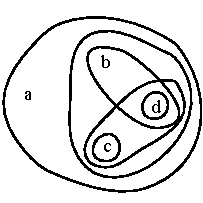
\includegraphics[width=0.3\textwidth]{example-topology.pdf}
    \end{center}
    \caption{odprte množice na končni množici $X$ iz primera \ref{ex1}}
\end{figure}
\begin{example}\label{ex1}
  Naj bo $(X,\mathcal{T})$ topološki prostor, pri čemer je $X = \{a,b,c,d\}$ končna
  množica, odprte množice pa so $\emptyset, \{a,b,c,d\}, \{b,d\}, \{c\}, \{d\},
  \{b,c,d\}$ in $\{c,d\}$. Prostor je $T_0$, torej je delno urejen. Slika \ref{pic1}
  \begin{figure}[h]
      \begin{center}
      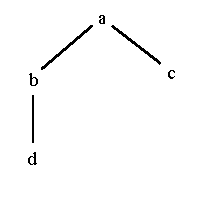
\includegraphics[width=0.3\textwidth]{hasse-example.pdf}
      \end{center}
      \caption{hassejev diagram končne delno urejene množice iz primera \ref{ex1}}
      \label{pic2}
  \end{figure}
    prikazuje odprte množice na $X$ z zaprtimi krivuljami.
    Ker je množica delno urejena, lahko prostor lepše predstavimo s Hassejevim diagramom (Slika \ref{pic2}).
    To lahko naredimo za vse končne $T_0$ prostore. Hassejev diagram je graf,
    kjer so vozlišča elementi množice, povezave pa urejeni pari $(x,y)$, kjer je $x < y$ in
    ne obstaja $z \in X$, da bi veljalo $x < z < y$. V diagramu
    bomo namesto puščice iz $x$ v $y$ narisali $y$ nad $x$.
\end{example}
\newpage
Na delni urejenosti definiramo nekaj izrazov.
Element $x$ je \textbf{maksimalen}, če $y \geq x$ implicira $y=x$, in je \textbf{maksimum} delne urejenosti, če velja
$y \leq x$ za vsak $y \in X$. Delna urejenost ima \textbf{maksimum}, če in samo če
obstaja natanko en maksimalen element. \textbf{Minimalen} element in \textbf{minimum} sta
definirana dualno.\\
\textbf{Veriga} v delni urejenosti je podmnožica elementov, ki so paroma primerljivi.
\textbf{Antiveriga} je podmnožica elementov, ki so paroma neprimerljivi.\\

%% flag complex
\section{Simplicialni kompleksi}
Celični kompleks je abstraktna struktura, ki je sestavljena iz celic in njihovih
relacij. Najprej si bomo ogledali tip celičnega kompleksa (simplicialni kompleks),
ki je bolj regularen in zaradi tega lažji za uporabo v računalništvu. V zadnjem 
razdelku \ref{celicni-kompleksi} bomo definirali splošnejši celični kompleks.\\
Simplicialni kompleks $K$ je sestavljen iz množic $V_K$ in $S_K$, pri čemer je
$S_K$ sestavljena iz končnih, nepraznih podmnožic množice $V_K$.
Množici $V_K$ pravimo množica točk, $S_K$ pa množica simpleksov. Veljati mora, da
je vsaka podmnožica $V_K$ moči 1 simpleks in da je vsaka neprazna podmnožica
simpleksov simpleks. Malce lahko zlorabimo notacijo in pišemo $v \in K$ namesto
$v \in V_K$ in $\sigma \in K$ namesto $\sigma \in S_K$. V večini primerov bomo
simplicialni kompleks identificirali samo z množico njegovih simpleksov.\\
Če je simpleks $\sigma$ podmnožica simpleksa $\tau$, pravimo, da je $\sigma$ njegovo \textbf{lice}.
Simpleks, ki ima $n+1$ točk, imenujemo \textbf{$n$-simpleks} in pravimo, da je \textbf{dimenzije} $n$.
Vse točke $K$ predstavljajo 0-simplekse. Dimenzija $K$ je supremum dimenzij
vseh simpleksov v $K$. Če je $K$ prazen, ima dimenzijo -1, če pa vsebuje $K$ simplekse
poljubno velike dimenzije, je njegova dimenzija neskončno.\\
Naj bo $\sigma = \{v_0,v_1,\dots,v_n\}$ simpleks dimenzije $n$. Zaprt simpleks
$\bar{\sigma}$ je množica konveksnih kombinacij točk v $\sigma$:
\[
  \bar{\sigma} = \left\{\sum_{i=0}^n \lambda_i v_i\ |\ \lambda_i \geq 0, \sum_{i=0}^n \lambda_i = 1\right\}
\]
Geometrijska realizacija $|K|$ simplicialnega kompleksa $K$ je množica 
vseh takih konveksnih kombinacij $\sum_{v\in K} \lambda_v v,\ \lambda_v \geq 0$, tako da vsi $v$, ki imajo
neničelno $\lambda_v$, tvorijo simpleks v $K$. $|K|$ je torej unija vseh zaprtih
simpleksov $K$.
\begin{example}
  Naj bo $K$ simplicialni kompleks, ki vsebuje simplekse
  $\{a,b,c\}$, $\{b,d\}$, $\{c,d\}$, $\{b,e\}$, $\{f\}$ in vse njihove neprazne
  podmnožice.
  Geometrijska realizacija $|K|$ je prikazana na sliki \ref{sx}.
  \begin{figure}[h]
      \begin{center}
      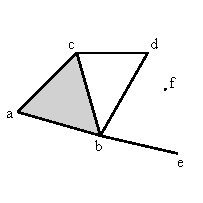
\includegraphics[width=0.4\textwidth]{simplicialni-kompleks.pdf}
      \end{center}
      \caption{geometrijska realizacija simplicialnega kompleksa $K$}
      \label{sx}
  \end{figure}
  Abstraktne konveksne kombinacije lahko vizualiziramo s konveksnimi kombinacijami
  točk, ki so v 'splošni legi'.
\end{example}
\newpage
Topološki prostor $X$ je \textbf{topološki polieder}, če obstaja simplicialni
kompleks $K$, da je $X$ homeomorfen telesu $|K|$. Simplicialni kompleks
$K$ imenujemo \textbf{triangulacija} poliedra $X$.
\begin{example}
  Pokažemo lahko, da je kolobar topološki polieder tako, da skiciramo njegovo
  triangulacijo.
    \begin{figure}[h]
        \begin{center}
        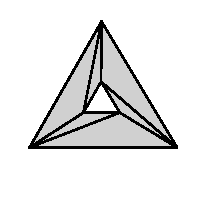
\includegraphics[width=0.4\textwidth]{torus-simpleks.pdf}
        \end{center}
        \caption{triangulacija kolobarja}
    \end{figure}
\end{example}
Za dan simplicialni kompleks $K$ konstruiramo njegovo \textbf{baricentrično subdivizijo} $K'$.
Točke $K'$ so simpleksi $K$ in simpleksi $K'$ so verige simpleksov $K$. Veriga
simpleksov je taka množica $\{\sigma_0,\sigma_1,\dots,\sigma_n\},\ \sigma_i \in K$
, da velja $\sigma_0 \subsetneq \sigma_1 \subsetneq \dots \subsetneq \sigma_n$.
\newpage
\begin{figure}[h]
  \begin{center}
  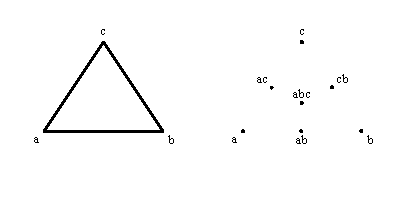
\includegraphics[width=0.8\textwidth]{baricentricna1.pdf}
  \end{center}
  \caption{prvi korak baricentrične subdivizije}
  \label{baricent1}
\end{figure}
\begin{figure}[h]
  \begin{center}
  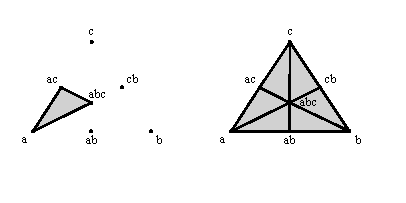
\includegraphics[width=0.8\textwidth]{baricentricna2.pdf}
  \end{center}
  \caption{simpleks $\{a, ac, abc\}$ in rezultat baricentrične subdivizije}
  \label{baricent2}
\end{figure}
\begin{example}
  Naj bo $K$ 2-simpleks $\{a,b,c\}$. Če hočemo konstruirati baricentrično subdivizijo $K$,
  moramo najprej dodati točke za vsak simpleks v $K$ (Slika \ref{baricent1}).
  Nato dorišemo še najdaljše verige, saj so v tem primeru vsi ostali simpleksi v $K'$ njihove podmnožice.
  Primer take verige je $\{a, ac, abc\}$, saj velja $a \subsetneq ac \subsetneq abc$ (Slika \ref{baricent2}).
\end{example}

\section{Povezava topoloških prostorov in simplicialnih kompleksov}
\begin{definition}
  Naj bo $X$ končni $T_0$ topološki prostor. Simplicialni kompleks $\mathcal{K}(X)$,
  asociiran z $X$, je simplicialni kompleks, katerega množica simpleksov so neprazne verige $X$.
\end{definition}
\begin{definition}\label{asociated-poset}
  Naj bo $K$ simplicialni kompleks. Asociirana delna urejenost $\mathcal{X}(K)$ je
  množica simpleksov $K$, urejena z relacijo inkluzije. Če sta $\sigma, \mathcal{T} \in K$,
  je $\sigma \leq \mathcal{T}$, če je $\sigma \subseteq \mathcal{T}$.
\end{definition}
Vidimo lahko tesno povezavo med topološkimi prostori, delnimi urejenostmi in
simplicialnimi kompleksi.
\begin{example}
Recimo, da je $K$ 2-simpleks $\{a,b,c\}$. Asociirana delna urejenost $\mathcal{X}(K)$
je množica simpleksov $K$, urejena z relacijo inkluzije. Na sliki \ref{baricent-asoc} je prikazan
Hassejev diagram asociirane delne urejenosti.
\begin{figure}[h]
  \begin{center}
  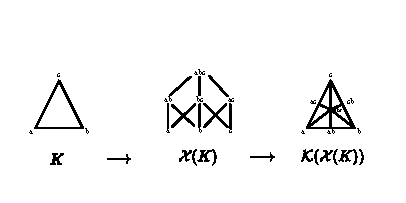
\includegraphics[width=1\textwidth]{baricent-asoc.pdf}
  \end{center}
  \caption{skica baricentrične subdivizije $\mathcal{K}(\mathcal{X}(K))$}
  \label{baricent-asoc}
\end{figure}
  Asociirana delna urejenost ima tudi
svoj simplicialni kompleks $\mathcal{K}(\mathcal{X}(K))$, kar je točno
baricentrična subdivizija $K$.
\end{example}

\chapter{Digitalni prostori}
Glavni cilj digitalne topologije in digitalne geometrije je premostiti vrzel
med geometrijskimi in topološkimi lastnosti komputacijskih objektov in njihovimi
teoretičnimi reprezentacijami v zveznem prostoru $\mathbb{R}^n$. Če hočemo uporabiti
topološke pojme v digitalni domeni, moramo najprej definirati prostor, ki je
analogen zveznemu prostoru $\mathbb{R}^n, (n > 1)$.\\
Ponavadi definiramo digitalne prostore na dva načina. Lahko se odločimo, katero 
vrsto povezanosti ima prostor. Naj bo $x = (x_1,\dots,x_n)$
točka v $\mathbb{Z}^n,\ n > 1$.\\
  ($3^n-1$)-sosed točke $x$ je vsaka točka
  $y = (y_1,\dots,y_n) \in \mathbb{Z}^n$, za katero velja
  \[
    \max|x_i - y_i| = 1 \text{.}
  \]
  Tak prostor bomo označili z $(d_{\inf},n)$-prostor.
  Recimo $(d_{\inf},2)$-prostor je 8-povezana mreža.\\
  $2n$-sosed točke $x$ je vsaka točka $y = (y_1,\dots,y_n) \in \mathbb{Z}^n,\ n > 1$,
  za katero velja
  \[
    \sum_{i=1}^{n}|x_i - y_i| = 1 \text{.}
  \]
  Tak prostor bomo označili z $(d_1,n)$-prostor.
  Recimo $(d_1,2)$-prostor je 4-povezana mreža.\\
  V razdelku \ref{obstoj} bomo pokazali, da 8-povezana mreža in s tem tudi
  $(d_{\inf},n)$-prostor nima kompatibilne topologije.

\section{Topologije na grafih}
\begin{definition}
  Za dan topološki prostor $(X, \mathcal{T})$ in dano podmnožico $S \subseteq X$ definiramo
  topologijo, zožano na $S$: \[\mathcal{T}|_S = \{U \cap S\ |\ U \in \mathcal{T}\}\]
\end{definition}
\begin{definition}
  Naj bo $G = (V,E)$ graf. Naj bo $\mathcal{T}$ topologija na $V$. $\mathcal{T}$ imenujemo \textbf{kompatibilna
  topologija} na $G$, če velja, da je
  $V' \subseteq V$ topološko povezan če in samo če je $G[V']$ grafovsko povezan.
\end{definition}
\begin{theorem}\label{theorem1}
  Naj bo $G$ graf s kompatibilno topologijo $\mathcal{T}$. Za vsak induciran podgraf
  $H \sqsubseteq G$ je topologija, omejena na $V(H)$, kompatibilna topologija
  na grafu $H$. To topologijo označimo z $O|_{V(H)}$.
\end{theorem}
\begin{proof}
  Za vsak $H' \sqsubseteq H$ imamo $\mathcal{T}|_{V(H)}|_{V(H')} = \mathcal{T}|_{V(H')}$. 
  Vsaka podmnožica $V(H)$ je povezana v $\mathcal{T}|_{V(H)}$, če in samo če je povezana v $\mathcal{T}$.
  $H' \sqsubseteq G$ je povezan, če in samo če je $V(H') \subseteq V(H)$ povezan v $\mathcal{T}$.\\
\end{proof}

\section{Kompatibilne topologije na dvodelnih grafih}
Naj bo $G^b$ povezan dvodelen graf $G^b = (V,E)$, ki ima vsaj tri vozlišča.
$V$ je torej unija dveh nepraznih disjunktnih množic $V_A$ in $V_B$. Vsaka
povezava v $E$ povezuje samo vozlišča iz $V_A$ z vozlišči iz $V_B$.\\
Definiramo dve kompatibilni topologiji na množici vozlišč $V$ tako, da opišemo
topološko okolico vsake točke $x \in V$. To je najmanjša odprta množica, ki
vsebuje $x$: $U_x \in \mathcal{T}$. Ker $U_x$ ni mogoče razdeliti na odprte množice, je $U_x$
in vsaka podmnožica $U_x$, ki vsebuje $x$, povezana.
Poleg tega je vsaka $U \in \mathcal{T},\ U \neq \emptyset$, unija določenih $U_x$.\\
Naj bo $N_x = \{y \  | \  yx \in E\}$ množica sosednjih točk točke $x$.\\
\[
  \begin{split}
  \mathcal{T}_1:&\quad
  U_x:=\{x\}\ \ \forall x \in V_A, \quad
  U_x:=\{x\}\cup N_x\ \  \forall x \in V_B\\
  \mathcal{T}_2:&\quad
  U_x:=\{x\}\cup N_x\ \  \forall x \in V_A, \quad
  U_x:=\{x\}\ \ \forall x \in V_B\\
\end{split}
\]
Kompatibilni topologiji $O_1$ in $O_2$ nista ekvivalentni, razen na grafih,
ki nimajo povezav; lahko nista niti homeomorfni.
\begin{theorem}
  $O_1$ in $O_2$ sta kompatibilni topologiji na $G^b$.
\end{theorem}
\begin{proof}
  Naj bo $\mathcal{T}$ enak $\mathcal{T}_1$ ali $\mathcal{T}_2$.
  \begin{itemize}
    \item[(1)] Naj bo $G' \sqsubseteq G^b$ povezan graf. Dokazati želimo, da je
    množica $V(G')$ povezana v $\mathcal{T}$, torej, da je ne moremo razdeliti na dve
    disjunktni odprti podmnožici. Za vsaki dve sosednji točki $x$ in $y$ je
    $U_x \cap U_y$ neprazen, saj $y \in U_x$ ali $x \in U_y$. $V(G')$
    razdelimo na dve neprazni disjunktni množici $V_1$ in $V_2$,
    $V(G') = V_1 \cup V_2$. Naj bo $A \in \mathcal{T}|_{V(G')}$
    najmanjša odprta množica, ki vsebuje $V_1$, in $B \in \mathcal{T}|_{V(G')}$
    najmanjša odprta množica, ki vsebuje $V_2$. Tedaj je $A \cap B \neq \emptyset$,
    torej je $V(G')$ povezan v $\mathcal{T}$.
    \item[(2)] Naj bo $G' \sqsubseteq G^b$ nepovezan graf. Dokazati želimo, da
    je množica $V(G')$ nepovezana v $\mathcal{T}$. Ker je $G'$ nepovezan, lahko $G'$ razdelimo
    na unijo dveh ne nujno povezanih induciranih podgrafov $C$ in $D$ tako, da nobeno vozlišče iz $C$
    ni povezano z nobenim vozliščem iz $D$. Torej
    \[\bigcup_{x\in V(C)}U_x \cap V(D) = \emptyset = V(C) \cap \bigcup_{x\in V(D)}U_x\]
    $V(C)$ in $V(D)$ lahko razpišemo:
    \[V(C) = V(G') \cap \left(\bigcup_{x\in V(C)} U_x\right)\]
    \[V(D) = V(G') \cap \left(\bigcup_{x\in V(D)} U_x\right)\]
    Vidimo, da sta $V(C)$ in $V(D)$ disjunktni odprti množici v $\mathcal{T}|_{V(G')}$,
    torej je $V(G')$ nepovezana v $\mathcal{T}$.
  \end{itemize}
\end{proof}

Naj bo $\mathcal{T}$ poljubna kompatibilna topologija na $G^b$. Naslednje leme držijo za vsak $x \in V$:
\begin{lemma}\label{lem1}
  $\{x\} \subseteq U_x \subseteq \{x\} \cup N_x$.
\end{lemma}
\begin{proof}
  $\{x\} \subseteq U_x$ sledi iz definicije. Recimo, da obstaja $x$, za katerega velja
  $U_{x} \nsubseteq \{x\} \cup N_{x}$. Potem obstaja
  $y \in U_{x}$, $y \notin \{x\} \cup N_{x}$. Ker je $\{x, y\} \subseteq U_x$,
  je ta množica povezana v $\mathcal{T}$. Ker je $G^b[\{x',y\}]$ nepovezan graf, je to v
  protislovju z definicijo kompatibilne topologije na $G^b$.
\end{proof}
\begin{lemma}\label{lem2}
  $U_x = \{x\}$ ali $U_x = \{x\} \cup N_x$.
\end{lemma}
\begin{proof}
  Recimo, da lema ne drži. Potem obstaja $x'$, da $U_{x'} \neq \{x'\}$ in
  $U_{x'} \subsetneq \{x'\} \cup N_{x'}$. Torej obstaja $y \in N_{x'}$, $y \notin U_{x'}$.
  Ker je $y \in N_{x'}$, sta $x$ in $y$ povezana. Ker sta povezana in je $G^b$
  dvodelen graf, velja $N_{x'} \cup N_y = \emptyset$. Ker sta $U_{x'}$ in $U_y$ 
  podmnožici $N_x'$ in $N_y$, je bodisi $U_{x'} \cap U_y = \emptyset$,
  bodisi $U_{x'} \cap U_y = \{x'\}$. Če velja $U_{x'} \cap U_y = \emptyset$, sledi
  protislovje, saj je $\{x',y\}$ povezana množica v $\mathcal{T}$.
  Če velja $U_{x'} \cap U_y = \{x'\}$, potem je $U_{x'} = \{x'\}$, kar je v
  protislovju s predpostavko $U_{x'} \neq \{x'\}$.
\end{proof}
\begin{lemma}\label{lem3}
  Naj bo $x \in V(G^b)$. Za vsak $y \in N_x$ velja $U_x = \{x\} \iff U_y = \{y\} \cup N_y$.
\end{lemma}
\begin{proof}
  Obravnavamo dve možnosti:
  \begin{itemize}
    \item[(1)] Naj bo $U_x = \{x\}$. Če je in $U_y = \{y\}$ za katerikoli $y \in N_x$, pridemo v protislovje, saj je 
    $\{x,y\}$ nepovezana v $\mathcal{T}$, $y$ pa je sosed $x$.
    \item[(2)] Naj bo $U_x = \{x\} \cup N_x$. Če velja $U_y = \{y\} \cup N_y$ za katerikoli $y \in N_x$, potem je
    $U_x \cap U_y = \{x, y\} \in \mathcal{T}$ (ker je $y \in N_x \Rightarrow x \in N_y$). Ker je
    $U_x$ najmanjša odprta množica, ki vsebuje $x$, je $U_x = \{x,y\}$. Prav tako je
    tudi $U_y = \{x,y\}$. Iz leme \ref*{lem2}, sledi, da je $N_x = \{y\}$ in $N_y = \{x\}$.
    Ker je graf povezan in je $y$ edini sosed $x$, sta ti dve točki cel graf
    $V(G^b) = \{x,y\}$, kar je v protislovju s predpostavko, da ima $G^b$ vsaj tri vozlišča.
  \end{itemize}
\end{proof}

Iz zadnje leme sledi spodnji izrek.
\begin{theorem}
Vsak povezan, dvodelen graf $G^b = (V,E)$, ki ima vsaj tri vozlišča, ima natanko
dve kompatibilni topologiji. To sta $\mathcal{T}_1$ in $\mathcal{T}_2$:
\[
  \begin{split}
  \mathcal{T}_1:&\quad
  U_x:=\{x\}\ \ \forall x \in V_A, \quad
  U_x:=\{x\}\cup N_x\ \  \forall x \in V_B\\
  \mathcal{T}_2:&\quad
  U_x:=\{x\}\cup N_x\ \  \forall x \in V_A, \quad
  U_x:=\{x\}\ \ \forall x \in V_B\\
\end{split}
\]
\end{theorem}

\section{Obstoj kompatibilne topologije na grafu} \label{obstoj}

\begin{corollary}\label{corollary1}
Cikel $C$, ki ima liho število vozlišč $n > 3$, nima kompatibilne topologije.
\end{corollary}
\begin{proof}
Za vsak $x \in V(C)$ je $G_x^b := C[\{x\} \cup N_x]$ dvodelen graf, ki ima vsaj tri
vozlišča. Recimo, da ima $C$ kompatibilno topologijo $\mathcal{T}$. Potem je na vsakem $G_x^b$ inducirana 
kompatibilna topologija $\mathcal{T}_1$ ali $\mathcal{T}_2$. Za vsaki dve sosednji točki $x,y \in V(C)$ velja
\[
  \mathcal{T}|_{V(G_x^b)} \cong \mathcal{T}_1 \iff \mathcal{T}|_{V(G_y^b)} \cong \mathcal{T}_2.
\]
sicer bi $U_x = \{x\}$ in $U_y = \{y\}$, kar bi pomenilo, da je množica
$\{x, y\}$ nepovezana v $\mathcal{T}$, kar to je v protislovju s predpostavko, da sta $x$ in
$y$ povezana. Če si izberemo neko začetno točko $X_0 \in V(C)$, lahko zaporedoma
izbiramo sosednje točke in opazujemo inducirane kompatibilne topologije:
\[\mathcal{T}|_{V(G_{X_0}^b)} \cong \mathcal{T}_1\]
\[\mathcal{T}|_{V(G_{X_1}^b)} \cong \mathcal{T}_2\]
\[\mathcal{T}|_{V(G_{X_3}^b)} \cong \mathcal{T}_1\]
Ker ima cikel liho število vozlišč, se na $x_0$ inducira kompatibilna topologija $\mathcal{T}_2$. Torej
sta na podgrafu $G^b_{x_0}$ inducirani tako $\mathcal{T}_1$ kot $\mathcal{T}_2$, kar ni mogoče.
\end{proof}

Iz posledice \ref*{corollary1} in iz Izreka \ref*{theorem1} sledi naslednji izrek.
\begin{theorem}
Naj bo $G$ graf v katerem obstaja induciran podgraf, ki je cikel lihe dolžine. Potem
$G$ nima kompatibilne topologije.
\end{theorem}
Zaradi izreka lahko sklepamo, da 8-povezana mreža nima kompatibilne topologije,
saj v njem obstaja induciran podgraf, ki je cikel lihe (Slika \ref{oddCircle}).
\begin{figure}
  \begin{center}
  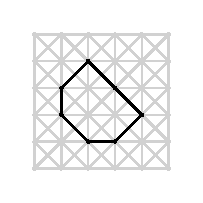
\includegraphics[width=0.4\textwidth]{odd_circle.pdf}
  \end{center}
  \caption{cikel lihe dolžine kot induciran podgraf 8-povezane mreže}
  \label{oddCircle}
\end{figure}
Mrežo lahko s pomočjo celičnih kompleksov malce drugače konstruiramo, tako
da bo imela kompatibilno topologijo.

\section{Celični kompleksi} \label{celicni-kompleksi}
Abstraktni celični kompleksi so podobni simplicialnim kompleksom, le da
celice poljubne oblike in relacije med njimi bolj splošne. Abstraktni celični kompleks
je trojica $C = (E,B,Dim)$, kjer je $E$ množica abstraktnih objektov (celic), $B \subseteq E \times E$ antisimetrična,
irefleksivna in tranzitivna relacija in $Dim:\ E \rightarrow I\subseteq\mathbb{N}$ funkcija
za katero velja: $Dim(e) < Dim(e')$ za vsak $(e,e') \subseteq E$. Tej funkciji pravimo
dimenzija.
\begin{figure}[h]
  \begin{center}
  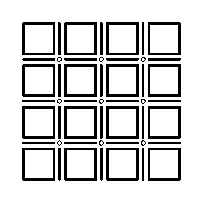
\includegraphics[width=0.4\textwidth]{r2-cell.pdf}
  \end{center}
  \caption{primer dela celičnega kompleksa}
  \label{celicni}
\end{figure}
Prostor $\mathbb{R}^2$ lahko predstavimo kot celični kompleks, kjer so celice
točke, daljice in ploskve. Relacijo $B$ definiramo kot relacijo, ki povezuje
točke in daljice, daljice in ploskve ter točke in ploskve. Dimenzija točke je 0,
dimenzija daljice je 1, dimenzija ploskve pa je 2. Skico lahko vidimo na sliki
\ref{celicni}.
Na podoben način, kot smo definirali asociirano delno urejenost s simplicialnim
kompleksom (Definicija \ref{asociated-poset}), lahko definiramo asociiran graf
$G(C)$ na sledeč način:
\begin{itemize}
  \item Vozlišča grafa so celice $E$.
  \item Povezava med dvema vozliščema $x$ in $y$ obstaja, če in samo če je
  $(x,y) \in B$ ali $(y,x) \in B$.
\end{itemize}
\begin{figure}[h]
  \begin{center}
  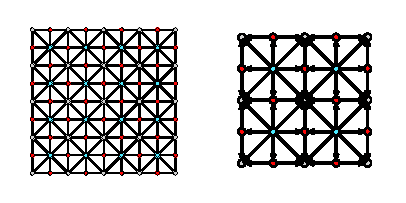
\includegraphics[width=1\textwidth]{r2-cell-graph.pdf}
  \end{center}
  \caption{levi del slike prikazuje induciran podgraf, asociiran s celičnim kompleksom
  iz slike \ref{celicni}, desni del papredstavlja orientacijo grafa}
  \label{celicni-graf}
\end{figure}
Na levem delu slike \ref{celicni-graf} je predstavljen del grafa, asociiranega s celičnim
kompleksom prostora $\mathbb{R}^2$. Siva vozlišča predstavljajo celice dimenzije 0, rdeča
vozlišča celice dimenzije 1, modra vozlišča pa celice dimenzije 2.
Ker je $B$ tranzitivna, je graf $G(C)$ graf primerljivosti. 
Relacijo lahko lepše prikažemo z orientacijo grafa $G(C)$, tako da za vsak
$(x,y) \in B$ narišemo povezavo iz $x$ v $y$ (Slika \ref{celicni-graf}).
\begin{note}
  Graf $G(C)$ je zelo podoben grafu 8-povezane mreže in zdi se, da vsebuje induciran
  podgraf, ki je cikel lihe dolžine, podobno kot na sliki \ref{oddCircle}. Iz tega
  bi lahko sklepali, da tak kompleks nima kompatibilne topologije. Cikel lihe dolžine
  na sliki \ref{fail-celicni-graf} je sicer podgraf $G(C)$, vendar ni induciran.
  Induciran podgraf vsebuje vse povezave med vozlišči, ne samo izbrane.
\end{note}
\begin{figure}[h]
  \begin{center}
  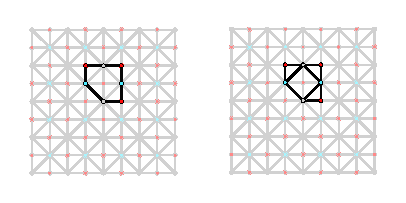
\includegraphics[width=1\textwidth]{odd-circle-r2-cell.pdf}
  \end{center}
  \caption{poskus iskanja cikla lihe dolžine v asociiranem grafu celičnega kompleksa}
  \label{fail-celicni-graf}
\end{figure}
S $H(X)$ označimo horizontalne sosede rdečega vozlišča $x$, z $V(x)$ pa vertikalne
sosede rdečega vozlišča $x$.\\
\begin{lemma}
  Naj bo $C$ celični kompleks prostora $\mathbb{R}^2$, in $\mathcal{T}$ $T_0$-Aleksandrova
  topologija, kompatibilna na $G(C)$. Za vsa vozlišča $x$ sive ali modre barve velja
  \[U_x = \{x\} \cup N_x \quad \text{ali} \quad U_x = \{x\}\text{.}\]
\end{lemma}
\begin{sketch}
Če velja $U_x \neq \{x\}$, lahko zaradi lastnosti $T_0$ pokažemo, da je šest od
osmih sosedov $x$ v $U_x$. Sklepamo lahko, da sta tudi ostala dva soseda v $U_x$.
Torej je $U_x = \{x\} \cup N_x$.
\end{sketch}

\begin{theorem}
  Naj bo $C$ celični kompleks prostora $\mathbb{R}^2$. Na grafu $G(C)$ obstajata
  natanko dve kompatibilni topologiji. To sta $\mathcal{T}_1$ in $\mathcal{T}_2$:
  \begin{itemize}
    \item $\mathcal{T}_1$:
      \begin{itemize}
        \item Naj bo $x$ vozlišče modre barve. Potem je $U_x = \{x\} \cup N_x$.
        \item Naj bo $x$ vozlišče rdeče barve. Potem je $U_x = H(x)$.
        \item Naj bo $x$ vozlišče sive barve. Potem je $U_x = \{x\}$.
      \end{itemize}
      \item $\mathcal{T}_2$:
      \begin{itemize}
        \item Naj bo $x$ vozlišče modre barve. Potem je $U_x = \{x\}$.
        \item Naj bo $x$ vozlišče rdeče barve. Potem je $U_x = V(x)$.
        \item Naj bo $x$ vozlišče sive barve. Potem je $U_x = \{x\} \cup N_x$.
      \end{itemize}
  \end{itemize}
\end{theorem}
Sledi iz izrekov 2-5 v izseku \Citet*{Bretto2007}.
Dokaz izreka je izven obsega tega dela.
\begin{theorem}
  Topologiji $\mathcal{T}_1$ in $\mathcal{T}_2$ sta homeomorfni.
\end{theorem}
\begin{proof}
Graf lahko vložimo v $\mathbb{Z}^2$ tako, da bo \textbf{rdeče vozlišče} na mestu $(0,0)$ (Slika \ref{cell-graph-symetrical}).
Množico vozlišč sedaj razpišemo v odvisnosti od barve vozlišč:
\begin{itemize}
  \item Vozlišča sive barve se nahajajo na lihih $x$ in sodih $y$ koordinatah:
  \[W=\{(2n+1, 2m)\ |\ n,m \in \mathbb{Z}\}\]
  \item Vozlišča rdeče barve se nahajajo na afinih premicah s smernim koeficientom 1:
  \[R=\{(n, m)\ |\ n+m=2k,k\in \mathbb{N}^*,n,m \in \mathbb{Z}\}\]
  \item Vozlišča modre barve se nahajajo na sodih $x$ in lihih $y$ koordinatah:
  \[M=\{(2n, 2m+1)\ |\ n,m \in \mathbb{Z}\}\]
\end{itemize}
\begin{figure}[h]
  \begin{center}
  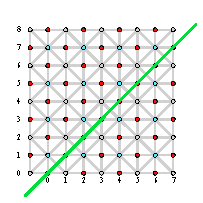
\includegraphics[width=0.6\textwidth]{r2-cell-graph-symetrical.pdf}
  \end{center}
  \caption{slika prikazuje simetrijo grafa $G(C)$, vloženega v $\mathbb{Z}^2$}
  \label{cell-graph-symetrical}
\end{figure}
Sedaj definiramo homeomorfizem:
\begin{align*}
    \phi:\ &(\mathbb{Z}^2,\mathcal{T}_1) \rightarrow (\mathbb{Z}^2,\mathcal{T}_2)\\
    &(x,y) \mapsto (y, x)
\end{align*}
Preslikava je zrcaljenje glede na premico $y=x$ (zelena premica na sliki \ref{cell-graph-symetrical}).
Pokazati moramo, da se okolica točke $(x,y)$ v $\mathcal{T}_1$ preslika v okolico točke $(y,x)$ v $\mathcal{T}_2$.
Okolico točke $a$ v $\mathcal{T}_1$ označimo z $U_{\mathcal{T}_1}(a)$.
Dokazati moramo torej
\[\phi(U_{\mathcal{T}_1}(x,y)) = U_{\mathcal{T}_2}((y,x))\text{.}\]
\begin{itemize}
\item[(1)] Naj bo $(x,y) \in R$ vozlišče rdeče barve. Ker velja $x+y = 2k = y+x$,
hitro vidimo, da je $(y,x) \in R$. Enako velja tudi za točke v okolici:
\begin{align*}
  \phi(U_{\mathcal{T}_1}((x,y))) &= \phi(H(X))\\
  &= \phi(\{(x+\epsilon,y), \epsilon \in \{-1,0,1\}\})\\
  &= \{(y,x+\epsilon), \epsilon \in \{-1,0,1\}\}\\
  &= U_{\mathcal{T}_2}((y,x))
\end{align*}
\item[(2)] Naj bo $(x,y) \in W$ vozlišče sive barve. Ker je $(x,y) = (2n+1, 2m)$,
je $(y,x) = (2m, 2n+1) \in M$. Okolica točke $(x,y)$ v $\mathcal{T}_1$ je samo točka $(x,y)$,
okolica točke $(y,x)$ v $\mathcal{T}_2$ pa je samo točka $(y,x)$.
\[
  \phi(U_{\mathcal{T}_1}((x,y))) = \phi(\{(x,y)\}) = \{(y,x)\} = U_{\mathcal{T}_2}((y,x))
\]
\end{itemize}
\end{proof}

\nocite{*}
\cleardoublepage
\addcontentsline{toc}{chapter}{Literatura}
\bibliography{literatura}
\bibliographystyle{plainnat}

\end{document}

